\pagestyle{MyStyle}

\chapter[GAMBA: an integrative platform for annotation of gene transcription-neuro- \\imaging associations]{GAMBA: an integrative platform for annotation of gene transcription-neuroimaging \\associations}

\chaptermark{GAMBA: a platform for annotation of transcription-imaging associations}

\label{ch:gamba}

\begin{refsection}

\begin{flushright}
\textit{Yongbin Wei, Siemon C. de Lange, Rory Pijnenburg, Lianne H. Scholtens, Dirk Jan Ardesh, Kyoko Watanabe, Danielle Posthuma, Martijn P. van den Heuvel}\\
Manuscript in preparation

\vspace{7 mm}

\end{flushright}
\newpage

\section*{Abstract}
The integration of neuroimaging and genetics enables us to assess the underlying biological mechanisms of human cognition and mental disorders. Here, we present a web-based application, GAMBA (short for Gene Annotation using Macroscale Neuroimaging Association), for scrutinizing gene transcription-neuroimaging associations. GAMBA utilizes gene expression data from the Allen Human Brain Atlas (AHBA) and cross-references the spatial pattern of cortical gene expression to the patterns of a range of neuroimaging-derived phenotypes. We present three examples to demonstrate the usability of GAMBA. In the first example, we show that brain expressions of human supragranular-enriched (HSE) genes are significantly correlated with the nodal strength of the macroscale brain connectome, suggestive of an association between micro- and macro-scale brain connectivity. The second and third examples show the expression profile of \textit{APOE} gene and risk genes for autism spectrum disorder (ASD) respectively to be associated with the pattern of brain structural and functional alterations in Alzheimer's disease and Asperger's syndrome. Together, GAMBA provides a user-friendly, open-source platform for functional annotation of genes concerning neuroimaging-derived phenotypes of the healthy and diseased brain.

\section*{Introduction}
Mapping the biological pathways that link genes with brain functions and dysfunctions enable us to formulate hypotheses on the mechanism of mental disorders and to prioritize genes for functional follow-up research.  The recent emergence of neuroimaging-genetic studies has described a growing number of genetic variants associated with multimodal neuroimaging traits by means of large-sample genome-wide association studies (GWAS)  \citep{elliott2018genome,Satizabal2019GeneticAO,Zhao2019GenomewideAA}. These neuroimaging traits have broadly covered anatomical morphology estimated by T1-weighted magnetic resonance imaging (MRI), brain activity measured using functional MRI (fMRI), and brain connectivity derived from diffusion weighted imaging and resting-state fMRI \citep{Miller2016MultimodalPB}. The single-nucleotide polymorphisms (SNPs) observed in GWAS are commonly assumed to play a role in encoding the amino acid sequences of proteins or regulating the activity of gene expression \citep{Shastry2009SNPsIO}, which in turn influences e.g. synaptic and neuron morphology, neuronal functioning, glial activity, et cetera, and ultimately the macroscale brain structure and function  \citep{Heuvel2019MultiscaleNO}. Empirical evidence for the associations between gene expression and the macroscale brain traits are however still largely missing.

Brain transcription data from the Allen Human Brain Atlas (AHBA) serves as a valuable quantitative reference to assess the transcription-neuroimaging linkage \citep{Hawrylycz2012AnAC}. Regional variation of gene expressions across the brain have been noted to often run parallel with spatial patterns of features derived from neuroimaging findings (see for reviews, \citep{Fornito2019BridgingTG,Heuvel2019MultiscaleNO}). Examples of these associations include genes related to oxidative metabolism to display transcriptional profiles in a similar pattern as the degree of inter-module long-distance functional connectivity (FC) \citep{vertes2016gene}, and genes enriched in supragranular layers of the human cortex to show transcriptional profiles that capture the architecture of both brain structural and functional networks \citep{krienen2016transcriptional,RomeroGarcia2018StructuralCN}. Transcriptional profiles of genes associated with human accelerated regions of the genome are also correlated to the pattern of cortical expansion in human evolution \citep{Wei2019GeneticMA}. Furthermore, brain transcriptional profiles of risk-genes related to brain dysfunction tend to show high similarity with disorder-specific brain changes revealed by neuroimaging techniques. Risk genes of schizophrenia and autism for example show elevated expression levels in brain areas where alterations of brain connectivity and morphology are evident \citep{romero2019synaptic,Romme2017ConnectomeDA} and gene markers for somatostatin interneurons are observed to be more expressed in cortical regions that are more vulnerable to major depressive disorder \citep{anderson2020convergent}.

Examining transcription-neuroimaging association based on spatial variations thus provides a unique opportunity for the exploration of genes related to specific phenotypes of cognitive abilities or brain disorders. Here, we present an integrative platform, GAMBA (short for Gene Annotation using Macroscale Neuroimaging Association) to scrutinize the potential transcription-neuroimaging associations. GAMBA is an open-access platform and is available online at \url{http://dutchconnectomelab.nl/GAMBA/} and can be directly used from the gene annotation application FUMA (\url{https://fuma.ctglab.nl/}) \citep{watanabe2017functional}. For any genes of interest, GAMBA displays the cortical expression profile of these genes derived from the AHBA dataset together with the spatial patterns of neuroimaging-related phenotypes, and accompanied statistical testing of the genetic-neuroimaging associations. Neuroimaging phenotypes include the topological layout of resting-state brain functional networks, brain structural connectivity, cognitive components, cortical metabolic properties, functional and structural alterations across a range of brain disorders, etcetera. GAMBA provides a user-friendly open-source platform for functional annotation of genes with respect to macroscale phenotypes of cognitive brain structure and function.

\section*{Results}
\subsection*{GAMBA overview}
GAMBA is built around the notion of cross-referencing human brain transcription data with the macroscale brain imaging data \citep{Anderson2018TheTL,krienen2016transcriptional,Romme2017ConnectomeDA,Wei2019GeneticMA}. Transcription data are obtained from the Allen Human Brain Atlas (AHBA; \url{http://human.brain-map.org}). Data preprocessing of the AHBA data includes gene information reannotation, probe selection, sample assignment, normalization, and averaging among brain donors (see Methods), resulting in the average transcriptional profile of 22,749 genes across 57 cortical areas of the left cortical mantle. The cortical expression profile of each of the 22,749 genes is linked to neuroimaging phenotypes from eight categories using a multivariate linear regression model (Figure \ref{gambaFig1}). Neuroimaging phenotypes include the spatial pattern of: a) resting-state functional networks \citep{thomas2011organization}, b) brain cognitive components \citep{Yeo2016GraphMO}, c) regional metrics derived from the brain structural and functional connectome, d) measurements of the level of cortical oxygen and glucose metabolism \citep{Vaishnavi2010RegionalAG}, e) human surface area expansion compared to the chimpanzee \citep{Wei2019GeneticMA}, f) brain volume alterations across twenty-two brain disorders \citep{Fox2002MappingCA,Fox2005BrainMapTO,Laird2005BrainMapT}, g) brain functional changes in sixteen brain disorders \citep{Fox2005BrainMapTO,Fox2002MappingCA,Laird2005BrainMapT}, h) brain dysconnectivity across nine psychiatric and neurological disorders \citep{Lange2019SharedVF}, i) brain functional correlates of 530 terms in relation to cognitive states and brain disorders, as described in the NeuroSynth database \citep{Yarkoni2011LargescaleAS}. Details about the datasets and statistical analyses are described in Methods.

In the following sections, we present three examples to demonstrate the validity of GAMBA and how GAMBA facilitates our understanding of the transcription-neuroimaging associations.


\begin{figure}[h]
    \centering
    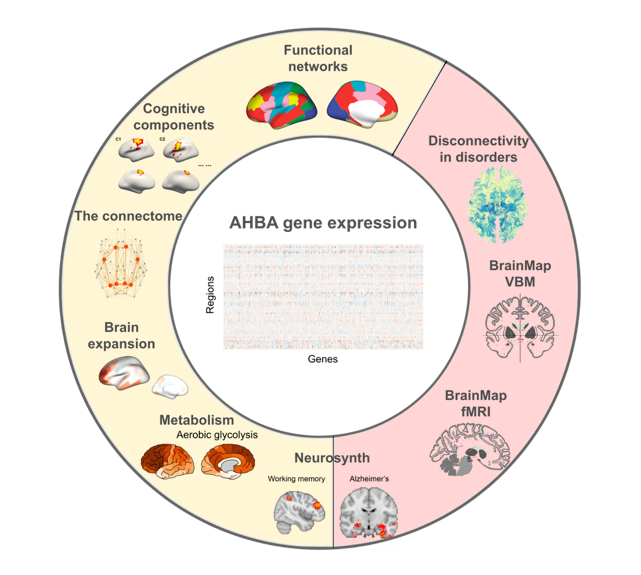
\includegraphics[width=10cm]{images/gambaFig1.png}
    \caption{An overview of the datasets used in GAMBA. Brain gene expressions are extracted from the Allen Human Brain Atlas (AHBA) and cross-reference to distinct brain imaging phenotypes. Yellow indicates brain imaging phenotypes related to healthy brain organization, red indicates brain imaging phenotypes related to brain disorders.}
    \label{gambaFig1}
\end{figure}

\subsection*{Application to genes related to neuronal connectivity}
As the first example, we apply GAMBA to genes related to the formation of microscopic neuronal connectivity, examining a set of 19 genes known to be enriched in supragranular layers of the human cerebral cortex (referred to as HSE genes) and known to play an important role in long-range cortico-cortical connections \citep{krienen2016transcriptional}. HSE genes showed significantly higher expression than genes on average in the inferior/superior parietal cortex, supramarginal cortex, precuneus, superior/middle frontal cortex, precentral gyrus, and paracentral cortex (Figure \ref{gambaFig2}a. , two-sided \textit{t}-test; \textit{q} < 0.05, False Discovery Rate [FDR] corrected). Lower HSE gene expression in comparison to genes on average was noted in the anterior cingulate gyrus, entorhinal cortex, parahippocampal gyrus, medial orbital frontal cortex, lingual gyrus, and insular (\textit{q} < 0.05, FDR corrected). Gene expression of HSE genes was significantly associated with the nodal strength of the structural connectome -- a measurement describing the extent to which a region is structurally connected to the rest of the brain [standardized beta (\textbeta) = 0.520, \pval < 0.001 for the connectivity weighted by the number of streamlines (NOS); \textbeta \ = 0.624, \pval < 0.001 for the connectivity weighted by streamline density (SD); FDR corrected; Figure \ref{gambaFig2}]. A similar correlation was shown between the gene expression profile of HSE genes and the nodal strength of the functional connectome (FC; \textbeta \ = 0.524, \pval < 0.001; FDR corrected; Figure \ref{gambaFig2}). These results suggest that the formation of microscale cortico-cortical connectivity is associated with the organization of macroscale connectome, stressing the usability of GAMBA to uncover the association across different scales of brain organization.

\begin{figure}[h]
    \centering
    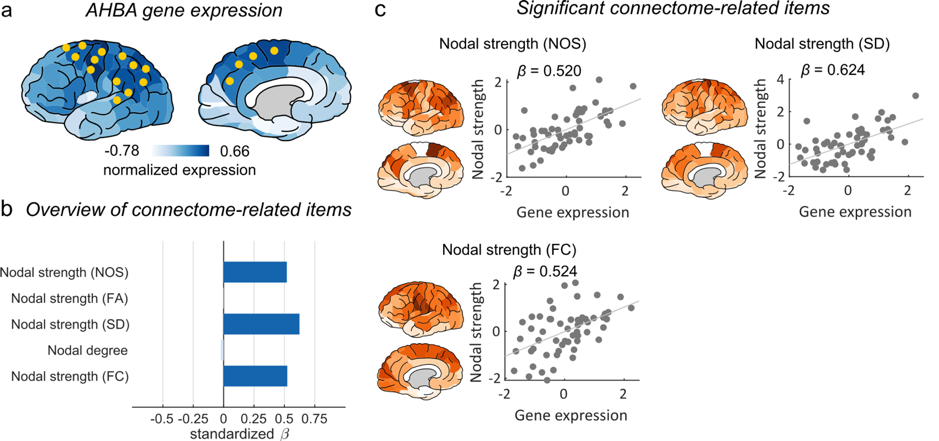
\includegraphics[width=\linewidth]{images/gambaFig2.png}
    \caption{Applications of GAMBA on HSE genes. (a) GAMBA figure panels of gene expression levels of HSE genes, showing significantly higher expressions of HSE genes than genes on average in the inferior/superior parietal cortex, supramarginal cortex, precuneus, superior/middle frontal cortex, precentral gyrus, and paracentral cortex. Yellow dots indicate significant regions (two-sided \textit{t}-test, \textit{q} < 0.05, FDR corrected). (b) GAMBA exhibits significant correlations between HSE gene expression and nodal strength of the structural (NOS-weighted, \textbeta \ = 0.520 and SD-weighted, \textbeta \ = 0.624) and functional connectome (\textbeta \ = 0.524; \textit{q} < 0.05, FDR corrected). (c) Brain maps of the significant brain imaging phenotypes, including the NOS-, SD-, and FC-weighted nodal strength, and scatter plots of the significant associations are displayed.}
    \label{gambaFig2}
\end{figure}

GAMBA includes null-models to disentangle functional annotations of genes of interest from effects present across all genes. GAMBA tests whether an observed association between gene expression of a set of genes (here HSE) and a macroscale phenotype of interest (here macroscale brain connectome measurements) is a general phenomenon that can be noted for all genes, or whether it is specific to the set of genes of interest. For this purpose, GAMBA uses bootstrap to estimate the mean and standard deviation of the effect size (\textbeta) for the same-sized gene-sets randomly selected from all genes (10,000 samplings; referred to as "NULL-1"). Performing \textit{z}-test showed that the observed effect size for associations between HSE genes and nodal strength weighted by NOS, SD, and FC were significantly larger than the mean effect size of all genes (NOS: \textit{z} \ = 3.874, \pval < 0.001; SD: \textit{z} \ = 3.492, \pval < 0.001; FC: \textit{z} \ = 2.408, \pval =  0.016; \textit{q} \ < 0.05, FDR corrected). 

GAMBA further includes more strict null-models (allowing for a more strict statistical evaluation) to compare the observed effect sizes to the mean effect size of a set of genes particular expressed in BRAIN tissues (referred to as "NULL-2") \citep{Wei2019GeneticMA}. Using this null-model showed significant associations between HSE genes and the connectome metrics (NOS: \textit{z} \ = 4.093, \pval < 0.001; SD: \textit{z} \ = 3.767, \pval < 0.001; FC: \textit{z} \ = 2.706, \pval =  0.007; FDR corrected).


GAMBA includes a third null-model to examine whether the observed association is independent of `generic anatomical relationships' across brain regions. For this, the gene expression data is rebuilt using randomized brain parcellations that are obtained by spinning the reconstructed sphere of the real brain parcellation (1,000 permutations; further referred to as "NULL-3", see Methods for details) as proposed by \citep{AlexanderBloch2018OnTF}, and all statistics are reperformed. Using this null model confirmed the significant association between expressions of HSE genes and structural connectivity strength (NOS: \textit{z} \ = 2.448, \pval =  0.007; SD: \textit{z} \ = 2.377, \pval =  0.009; FDR corrected), as well as the strength of functional connectivity (\textit{z} \ = 2.853, \pval =  0.002; FDR corrected). These GAMBA findings implicate a specific role of HSE genes in forming the neurons in supragranular layers and their cortico-cortical connectivity, which are the "building blocks" for the macroscale brain connectivity.


\subsection*{Application to Alzheimer's Disease Risk Gene APOE}
In the second example, we show the usability of GAMBA in examining brain patterns of disease-related pathology. We examine the Apolipoprotein E (APOE) gene, widely indicated as a risk gene for Alzheimer's disease (AD) \citep{Liu2013ApolipoproteinEA}. We hypothesize that the cortical gene expression of \textit{APOE} would be related to the cortical alterations revealed in patients with AD. First, GAMBA analysis showed the highest expression level of \textit{APOE} in the entorhinal cortex (\textit{z} \ = 2.092, \pval =  0.036; two-sided \textit{z}-test based on NULL-1; Figure \ref{gambaFig3}a), a region well-known to be involved in AD (Bobinski, et al., 1999) and often marked as one of the epi-centers of brain pathology in AD (Van Hoesen, et al., 1991). GAMBA analysis further showed significant associations between the transcriptional profile of \textit{APOE} and the cortical atrophy patterns as reported by the meta-analysis of BrainMap voxel-based morphometry (VBM) studies of i) Alzheimer's disease (\textbeta \ = 0.608, \pval < 0.001), ii) dementia (\textbeta \ = 0.621, \pval < 0.001), iii) semantic dementia (\textbeta \ = 0.587, \pval < 0.001), iv) frontotemporal dementia (\textbeta \ = 0.455, \pval < 0.001), v) attention deficit hyperactivity disorder (ADHD, which is hypothesized to be a risk factor of dementia pathology (Callahan, et al., 2017), \textbeta \ = 0.384, \pval =  0.002), and vi) bipolar disorder (\textbeta \ = 0.343, \pval = 0.010; \textit{q} \ < 0.05, FDR corrected; Figure \ref{gambaFig3}b). These effect sizes exceeded the null distributions of NULL-1 (i.e., mean effect sizes across all genes) for semantic dementia (\textit{z} \ = 2.019, \pval =  0.044) and Alzheimer's disease (\textit{z} \ = 2.039, \pval =  0.042). Examining spatial specificity showed significant associations of APOE's expression with brain volume changes in dementia (\textit{z} \ = 3.234, \pval =  0.001, NULL-3), Alzheimer's disease (\textit{z} \ = 3.119, \pval =  0.001 NULL-3), and frontotemporal dementia (\textit{z} \ = 2.785, \pval =  0.005; FDR corrected, NULL-3). NULL-2 (i.e., comparing the observed effect size to the mean effect size of brain-expressed genes, instead of ALL genes) did not reveal specific significant associations (\pval > 0.097), suggesting that there are other brain-expressed genes showing similar expression patterns to the atrophy pattern of above-mentioned diseases. 

Furthermore, cross-referencing transcription data to items in the functional NeuroSynth database again revealed significant associations of \textit{APOE} expression with terms of "Alzheimer" (\textbeta \ = 0.479, \pval < 0.001) and "dementia" (\textbeta \ = 0.451, \pval < 0.001; \textit{q} \ < 0.05, FDR corrected). 

\begin{figure}[h]
    \centering
    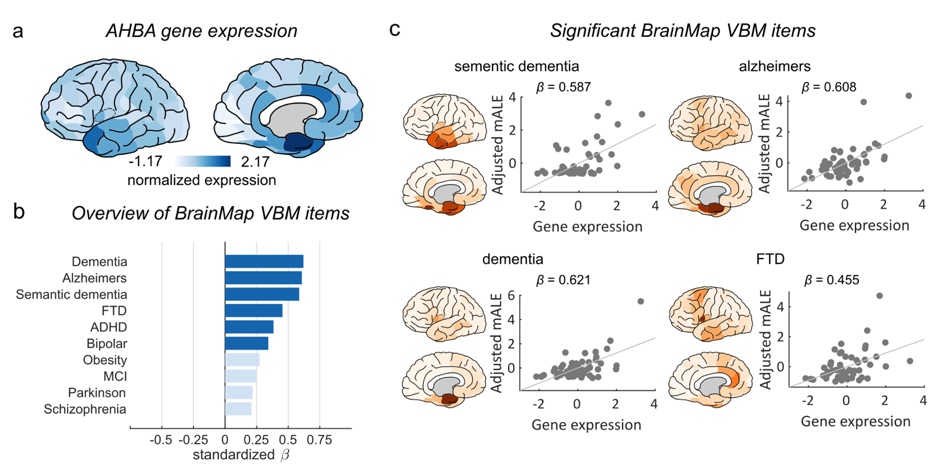
\includegraphics[width=\linewidth]{images/gambaFig3.png}
    \caption{Applications of GAMBA on \textit{APOE}. (a) GAMBA figure panels of gene expression levels of \textit{APOE}. (b) GAMBA analysis demonstrates significant correlations between \textit{APOE} gene expression and voxel-based morphometry (VBM) changes in sementic dementia (\textbeta \ = 0.587), alzheimers (\textbeta \ = 0.608), dementia (\textbeta \ = 0.621), frontotemporal dementia (\textbeta \ = 0.455). ADHD (\textbeta \ = 0.384), and bipolar disorder (\textbeta \ = 0.343; \textit{q} \ < 0.05, FDR corrected). (c) Brain maps of the significant brain imaging phenotypes, including the semantic dementia, Alzheimers, dementia, and frontotemporal dementia, and scatter plots of the significant associations (items showing significance for at least one NULL-model) are displayed.}
    \label{gambaFig3}
\end{figure}

GAMBA mapping further revealed a significant association of the transcriptional profile of \textit{APOE} with the organization of the limbic network (\textbeta \ = 0.532, \pval < 0.001; FDR corrected, \textit{q} \ < 0.05), exceeding the mean effect size of NULL-1 (\textit{z} \ = 2.260, \pval =  0.024) and NULL-3 (\textit{z} \ = 2.852, \pval =  0.004), but not the more strict NULL-2 (\textit{z} \ = 1.840, \pval =  0.066). We argue that these findings strengthen the importance of including a NULL-2 (i.e., null model of effect sizes of BRAIN genes), on top of the NULL-1 model \citep{romero2019synaptic,Romme2017ConnectomeDA}, in examinations of spatial correlations between transcription and imaging features. NULL-2 \citep{anderson2020convergent,Wei2019GeneticMA} is a more strict null model to avoid false-positive findings of gene-expression-neuroimaging associations. 

Taking together, our findings show that medial temporal and parahippocampal regions with high normative \textit{APOE} expression also display significantly elevated structural and functional brain abnormalities in dementia and AD in disease conditions. GAMBA gene mapping further suggests an important role of \textit{APOE} in regions of the limbic network, a network that is known to subserve brain functions of memory and emotion \citep{Catani2013ARL} and to be regularly reported to AD and MCI pathology and clinical outcome \citep{Nestor2003LimbicHI}.

\subsection*{Application to risk genes of autism}
We next apply GAMBA to risk genes of autism spectrum disorder (ASD) to further demonstrate the utility of the platform. A set of 25 ASD risk genes was obtained from a recent meta-analysis of genome-wide association study on 18,381 ASD cases and 27,969 controls \citep{Grove2019IdentificationOC}, 24 of which are included in the AHBA data (further referred to as ASD genes, averaged gene expression levels displayed in Figure \ref{gambaFig4}a). GAMBA analysis indicated high expression of ASD genes in the superior parietal lobe (\textit{z} \ = 2.654, \pval =  0.008), precuneus (\textit{z} \ = 2.304, \pval =  0.021), cuneus (\textit{z} \ = 2.684, \pval =  0.007), lingual gyrus (\textit{z} \ = 2.591, \pval =  0.010), lateral occipital lobe (\textit{z} \ = 2.573, \pval =  0.010), and pericalcarine (\textit{z} \ = 2.909, \pval =  0.004; uncorrected; two-sided \textit{z}-test comparing the NULL-1, Figure \ref{gambaFig4}a). This transcriptional profile showed a significant association with brain functional alterations as reported by the meta-analysis of BrainMap fMRI studies in "Asperger's syndrome" (\textbeta \ = 0.443, \pval < 0.001; FDR corrected) (Figure \ref{gambaFig4}b), a major diagnosis of ASD with difficulties in social interaction and nonverbal communication as derived from BrainMap data \citep{Fox2002MappingCA,Fox2005BrainMapTO,Laird2005BrainMapT}. The observed effect size was significantly larger than NULL-2 (\textit{z} \ = 2.097, \pval =  0.036) and NULL-3 (\textit{z} \ = 3.120, \pval =  0.002).

GAMBA further subdivided the 24 ASD genes in to four communities according to their co-expression network [Modularity index \textit{Q} = 0.243 (see methods), which was significantly different from the null distribution of modularity index derived from random genes (\pval = 0.001, 10,000 permutations)]. Two communities, including seven genes (\textit{HDAC4, KANSL1, KIZ, PLEKHM1, WDPCP, WNT3, XRN2}) and seven genes (\textit{CRHR1, MDH1, MFHAS1, NTM, PINX1, SOX7, XKR6}), separately, showed significant association with brain functional alterations as observed in "Asperger's syndrome" (\textbeta \ = 0.417, \pval =  0.002 and \textbeta \ = 0.407, \pval =  0.002; Figure \ref{gambaFig4}c). GAMBA findings thus suggest that cortical areas with high expression of ASD risk genes are more likely to show structural and functional brain alterations related to Asperger's syndrome, a condition strongly related to ASD \citep{Segal2010DiagnosticAS}.

\begin{figure}[h]
    \centering
    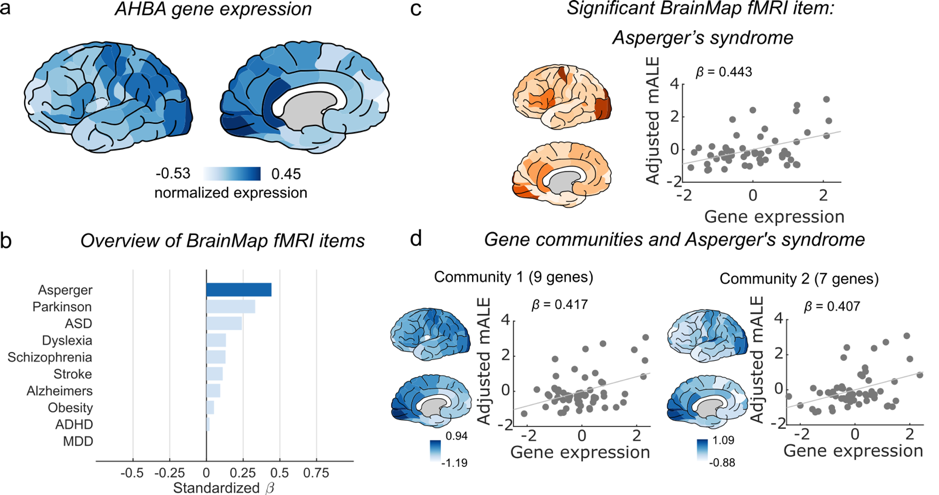
\includegraphics[width=\linewidth]{images/gambaFig4.png}
    \caption{Applications of GAMBA on ASD genes. (a) GAMBA figure panels of gene expression levels of ASD genes. (b) GAMBA demonstrates significant correlations between gene expression of ASD genes and brain activity changes in Asperger's syndrome (\textbeta \ = 0.444; \textit{q} \ < 0.05, FDR corrected). (c) Maps of brain activity changes in Asperger's syndrome and its association between ASD gene expression. (d) GAMBA detects communities within the set of ASD genes and shows two communities to be significantly correlated to brain activity changes in Asperger's syndrome (\textbeta \ = 0.417 and 0.407, separately).}
    \label{gambaFig4}
\end{figure}


\section*{Discussion}

The present study introduces a web-based application – GAMBA – that can be used to probe the association between transcription and brain structure/function derived from a wide range of neuroimaging data. Given a single gene or a set of genes, GAMBA tests whether brain regions in which genes of interest are preferentially expressed show overlapping patterns of a wide range of brain imaging phenotypes. 

The application of GAMBA is demonstrated in three examples, HSE genes, APOE, and ASD genes, showing GAMBA as a tool for gene function annotation in the context of both health and disease conditions. The applications we show for example indicate that the cortical transcriptional profile of genes involved in microscale neuronal connectivity runs parallel with variation in structural and functional connectivity across brain regions. HSE genes are known to be enriched in supragranular layers of the human cortex and are responsible for long-range corticocortical projections of pyramidal neurons \citep{Zeng2012LargeScaleCG}. Cortical transcriptional profiles of these genes capture the architecture of distributed brain functional networks \citep{krienen2016transcriptional} and correlate with the pattern of cortical thickness covariance network \citep{RomeroGarcia2018StructuralCN}. These findings suggest a putative role of HSE genes in shaping large-scale brain connectome, which is compatible with observations of association areas to display the more complicated dendritic structure of layer III pyramidal neurons and to be more connected by white matter tracts at the macroscale level of the connectome organization \citep{Scholtens2018MultimodalCI,Heuvel2019MultiscaleNO}. GAMBA analysis of HSE genes provides a new way of easily assessing such cross-scale associations of brain connectivity.

The utility of GAMBA is further shown in the application of disease conditions. \textit{APOE} gene expression pattern across cortical areas is shown to correlate with the patterns of structural and functional brain alterations in AD. The \textit{APOE} ε4 variant is known as one of the strongest genetic risk factors for late-onset AD \citep{Jansen2019GenomewideMI,Liu2013ApolipoproteinEA,Karch2015AlzheimersDR}. AD patients are known to have elevated expression levels of the \textit{APOE} gene in the hippocampus and medial temporal regions, areas that are well-known to be involved in the pathology of the disorder \citep{Akram2012AssociationOA,Linnertz2014TheCE,Matsui2007ExpressionOA}. Brain imaging studies have further shown that \textit{APOE} ε4 carriers show a larger extent of atrophy in these brain areas compared to healthy aging \citep{Agosta2009ApolipoproteinEE,Cacciaglia2018EffectsOA,Manning2014APOEI}. GAMBA analysis may further extend these findings by stressing that high normative levels of \textit{APOE} expression in for example medial temporal regions may be related to a higher risk for atrophy of these brain regions in AD pathology.

As for a third example we present an association between ASD risk genes and brain functional alterations in Asperger's syndrome that is part of the diagnosis of ASD. ASD is a highly heterogeneous disorder and patients with Asperger's syndrome are the subtype showing the highest heritability \citep{Grove2019IdentificationOC}. Our example adds to this by showing that genetic variants observed in ASD might be related to the vulnerability of brain functions in Asperger's syndrome. This finding is also in line with the observed association between ASD polygenic risk score and grey matter volume \citep{Ranlund2018AssociationsBP}, pointing to the contribution of genetic variants in macroscopic brain alterations reported in the disease. On top of that, this example shows the usage of GAMBA in post-GWAS analysis -- exploring brain-related functional annotation for genes identified in GWAS studies. 

GAMBA complements other tools that link genetics and brain functions. Tools like Neurosynth \citep{Yarkoni2011LargescaleAS} and Brain Annotation Toolbox \citep{Liu2019BrainAT} provide platforms to visualize the whole-brain map of gene expressions of a given gene and the maximal correlations between gene expressions and brain maps. GAMBA adds to this by integrating a large gene set or a broader range of brain imaging findings and by performing statistical evaluations of resulting associations. GAMBA is developed to provide a more complete inclusion of brain imaging findings across a wide range of modalities and datasets, and a quick, user-friendly, web-based interface. 

A number of methodological considerations have to be kept in mind when interpreting findings from GAMBA. First, GAMBA is based on gene expression data from the AHBA dataset, which were collected from post-mortem brain tissues from six human donors. Inter-individual gene expression variability is inherently not taken yet into account \citep{Miller2014TranscriptionalLO,Tebbenkamp2014TheDT}. As an integrative platform, GAMBA will allow for extensions of other datasets of brain gene expressions, such as PsychENCODE \citep{wang2018comprehensive} and BrainSpan \citep{johnson2009functional}. Second, AHBA gene expression data are extracted from post-mortem human brains with no psychiatric and neurologic conditions. Therefore, GAMBA results regarding brain disorders should be interpreted in the context of gene expression of risk genes in brain regions to be a potential marker for a higher susceptibility of these regions in relevant brain disorders \citep{McColgan2018BrainRS,Romme2017ConnectomeDA}. Third, GAMBA detects spatial associations between cortical gene expression profile and brain imaging findings, making it hard to directly infer causal relationships. GAMBA is best used to examine brain annotations of genes with hypothesized functions. Functional animal follow-up studies aiming to provide causal relations from gene expression and brain function and structure are needed. 

In conclusion, GAMBA provides a user-friendly platform to annotate transcriptome-neuroimaging associations, integrating brain gene expression data with a wide range of neuroimaging data. GAMBA can be used to gain new insights into brain-relevant functional annotations for genes of interests in relation to healthy brain structure and function, and in relation to structural and functional brain alterations across various brain disorders. By linking transcriptomic and neuroimaging data, GAMBA may help post-GWAS gene annotation, facilitating the prioritization of genes for further functional follow-up experiments. 

\section*{Methods}

\subsection*{Gene expression}
Microarray gene expression data were obtained from the Allen Human Brain Atlas (\url{http://human.brain-map.org}), with data collected from six postmortem brains of human donors without any neuropathological or neuropsychiatric conditions (demographics tabulated in Chapter \ref{ch:HAR}). Microarray analyses are described in detail in \url{http://help.brain-map.org/display/humanbrain/Documentation}. An average of 466 brain tissue samples in left hemisphere were obtained from four donors (466 $\mathsf{\pm}$ 72.6 samples from H0351.1009, H0351.1012, H0351.1015, and H0351.1016), and 946 and 893 samples covering both hemispheres from the remaining two donors (H0351.2001 and H0351.2002). We included tissue samples in cortical and subcortical regions of the left hemisphere and used the expression of 58,692 probes for each brain donor \citep{Romme2017ConnectomeDA,Wei2019GeneticMA}.

We performed probe-to-gene re-annotations using the BioMart data mining tool (\url{https://www.ensembl.org/biomart/}) \citep{Arnatkeviciute2019APG}. Gene symbols were replaced by the previous and alias gene symbols by the approved symbols obtained from the HUGO Gene Nomenclature Committee (HGNC) database (\url{http://biomart.genenames.org/}), resulting in the inclusion of 22,749 genes. Per brain, and per tissue sample, expressions of probes annotated to the same gene symbol were averaged, followed by log2 transformation with pseudocount 1. Tissue samples were spatially mapped to the FreeSurfer cortical regions to obtain region-wise gene expression profiles \citep{French2015AFV}. The cortical parcellation of 114 regions (57 per hemisphere) based on the Desikan-Killiany atlas (DK-114) was obtained for the Montreal Neurological Institute (MNI) ICBM152 template using FreeSurfer \citep{CAMMOUN2012386,DESIKAN2006968,FISCHL2012Freesurfer,Fonov2011UnbiasedAA,Fonov2009UnbiasedNA}. Brain tissue samples were annotated based on MNI coordinates to cortical regions in the DK-114 atlas by computing the nearest gray matter voxel in the MNI ICBM152 template in the FreeSurfer space. Tissue samples with a distance shorter than 2mm to the nearses gray matter voxel were included. Gene expression profiles of tissue samples belonging to the same cortical region were averaged, resulting in a 6 × 57 × 22,749 data matrix (i.e., donors × cortical regions × genes). Gene expression was normalized within each donor to \textit{z}-scores across all cortical regions per gene. Normalized gene expression profiles were averaged across the six donors obtaining a group-level gene expression matrix of size of 57 × 22,749. The resulting cortical patterns of expression of each gene was linked to the patterns of various neuroimaging findings as described in the following sections.


\subsection*{Resting-state functional networks}
Cortical regions in the DK-114 atlas were assigned to seven well-defined functional networks \citep{Power2011FunctionalNO,smith2009correspondence,thomas2011organization} using the Yeo 7-network atlas \citep{thomas2011organization}. Networks included the visual, somatomotor, dorsal-attention, ventral-attention, limbic, frontal-parietal, and default-mode network. Surface-based annotation of the functional networks of the averaged subject in FreeSurfer (i.e., fsaverage) was translated to a 3D brain image in volumetric space, in which each gray matter voxel was annotated to a network label. Per DK region the ratio of voxels that belonged to each of the seven functional networks was computed, resulting in a mapping matrix of the size of 114 × 7 to indicate the involvement of each DK region in each of the functional networks.

\subsection*{Brain cognitive components}
Brain regions were mapped to functional ontology of twelve distinct brain cognitive components related to various cognition and behavioral processes based on functional neuroimaging data from 10,449 experiments \citep{Yeo2016GraphMO}. Brain components on the averaged subject in FreeSurfer were downloaded from \url{ https://surfer.nmr.mgh.harvard.edu/fswiki/BrainmapOntology\_Yeo2015} and translated to 3D brain images in volumetric space. A mapping matrix of the size of 114 × 12 was computed indicating the level of involvement of each of the 114 cortical areas in each of the twelve cognitive components.

\subsection*{The connectome}
The human structural connectome was reconstructed using T1-weighted and diffusion-weighted MRI (dMRI) data of 487 subjects (age [mean $\mathsf{\pm}$ standard deviation]: 29.8 $\mathsf{\pm}$ 3.4 years old) from the Human Connectome Project \citep{VANESSEN201362}. White matter tracts were reconstructed from the dMRI data using deterministic tractography \citep{VANDENHEUVEL2016293,WEI2019bigbrain}. The 18 sets of b = 0 volumes were averaged, and the 270 diffusion images were realigned and corrected for motion and gradient-induced distortions \citep{ANDERSSON2002177}. The diffusion profile within each voxel was reconstructed using generalized q-sampling imaging (GQI) \citep{YEH2010} and deterministic tractography was used to reconstruct white matter tracts, performing fiber assignment using the Fiber Assignment by Continuous Tracking (FACT) algorithm \citep{MORI1999}. Eight streamline seeds were started per voxel and tracking was stopped if the streamline reached a voxel of low preferred diffusion direction [fractional anisotropy (FA) < 0.1], exited the gray matter/white matter mask, or made a sharp turn (> 45°). Next, a structural connectome was generated from the set of reconstructed tractography streamlines and the cortical parcellation of each subject. The number of streamlines (NOS), streamline density (SD),  mean fractional anisotropy (FA) were extracted and used as the weight of structural connectivity between cortical regions. A group-averaged binary network was formed by averaging values across subjects for connections observed in more than 60\% of the subjects \citep{Reus2013EstimatingFP}. Nodal degree was calculated as the number of connections linked to each region. Nodal strength was computed for each cortical region by summing up the weights of all connections linked to that region.

A functional connectome map was constructed using resting-state fMRI data. Data were realigned and co-registered with the T1-weighted image to overlap with the cortical parcellation maps. Blood oxygenation level-dependent (BOLD) time series were corrected for linear trends, as well as global nuisance covariance, including six head motion parameters and mean signals of white matter and the ventricles. We performed band-pass filtering (0.01-0.1 Hz) together with motion scrubbing to minimize the influence of head-motion \citep{Power2012SpuriousBS}. Regional time series were computed from the preprocessed fMRI data by averaging the time-series of all voxels within a cortical region. Interregional functional connectivity was calculated as Pearson's correlation coefficient between the time series of cortical regions. Negative correlations were excluded, and correlation coefficients were transformed to \textit{z}-scores using Fisher transformation. A group-level functional network was constructed by averaging \textit{z}-scores across all subjects. Nodal strength of functional connectivity was subsequently computed.



\subsection*{Resting cortical metabolism}

We used data of five cortical metabolic measurements obtained from positron emission tomography (PET) imaging (tabulated and described in detail in \citep{Vaishnavi2010RegionalAG}), including the vertebral metabolic rate for oxygen (CMRO2), cerebral metabolic rate for glucose (CMRGlu), glycolytic index (GI), oxygen-glucose index (OGI), and cerebral blood flow (CBF). Data of metabolic measurements were given based on the Brodmann atlas (BA) and were transformed to the DK-114 atlas using the following steps. We extracted the MNI coordinates of all gray matter voxels of the fsaverage subject in FreeSurfer and mapped MNI coordinates to the Talairach atlas to obtain the annotation of BA area, using the BioImage Suite (\url{https://bioimagesuiteweb.github.io/webapp/mni2tal.html}) \citep{Lacadie2008MoreAT}. With the resulting annotations, we assigned the value of metabolic measurements to each voxel in the gray matter of the fsaverage subject. For each region of the DK atlas mean values were calculated per metabolic measurement, among all gray matter voxels within that region, yielding a 114 × 5 data matrix of metabolic measurements.

\subsection*{Cortical expansion}
A brain map of evolutionary cortical expansion was obtained from \citep{Wei2019GeneticMA}, where T1-weighted MRI data from 29 chimpanzees and 50 humans were utilized to compute the surface area expansion of each homologous cortical region in the DK-114 atlas. The expansion was computed as (AREA\textsubscript{human} – AREA\textsubscript{chimpanzee}) / AREA\textsubscript{chimpanzee}. 

\subsection*{Anatomical and functional involvement in brain diseases}
The BrainMap database (\url{http://www.brainmap.org/}) containing published functional and structural neuroimaging experiments with coordinate-based results was used to extract brain mappings of a wide range of psychiatric and neurologic disorders. MNI coordinates related to 22 brain disorders from the voxel-based morphometry (VBM) database (Number of experiments = 46 $\mathsf{\pm}$ 48, ranges from 4 to 206) and of 16 brain disorders from the functional database (Number of experiments = 69 $\mathsf{\pm}$ 69, ranges from 13 to 267) were obtained using Sleuth \citep{Fox2005BrainMapTO,Fox2002MappingCA,Laird2005BrainMapT,Vanasse2018BrainMapVA}. Meta-analysis was performed for each disorder using activation likelihood estimation (ALE) implemented in GingerALE \citep{Eickhoff2009CoordinatebasedAL,Turkeltaub2012MinimizingWA}. ALE maps were registered to the MNI152 template in the FreeSurfer space using FLIRT \citep{JENKINSON2001143,JENKINSON2002825}. Furthermore, ALE scores of gray matter voxels within each DK region were averaged, resulting in two matrices with the size of 114 × 22 and 114 × 16, indicating the cortical involvement of each disorder anatomically or functionally.

\subsection*{Neurosynth data}
The Neurosynth database includes brain images generated using text-mining, meta-analysis and machine-learning techniques on MRI studies mapping the involvement of brain regions in a large variety of cognitive tasks and states (\url{http://www.neurosynth.org}) \citep{Yarkoni2011LargescaleAS}. We downloaded the brain mappings of 749 terms, with voxel-wise \textit{z}-scores representing the extent to which a voxel is associated with the corresponding term (FDR corrected, \textit{q} \ < 0.01). Images of 457 terms with abstract meaning (e.g., "association"), or with names of brain anatomy (e.g., "putamen") were excluded. Resulting 292 images were registered to the MNI152 template in FreeSurfer space using FLIRT \citep{JENKINSON2001143,JENKINSON2002825}. Average \textit{z}-score within each cortical region of the DK-114 atlas was computed, resulting in a 114 × 292 matrix to indicate the cortical involvement in each term.

\subsection*{Statistics}
We assessed the association between the cortical gene expression profile and the pattern of neuroimaging phenotypes using linear regression with cortical volume of each region (measured on the basis of the fsaverage subject in FreeSurfer) taken as a covariate:

\[
\mathsf{ Y_{i}= \beta_{0}+ \beta_{1}X_{j}+ \beta _{2}cov+ \varepsilon } 
\] 
\noindent
where \textit{Y}\textsubscript{i} indicates the normalized gene expression profile of gene \textit{i} or the averaged profile of\textit{ a gene set i}, \textit{X}\textsubscript{j} the standardized cortical profile of neuroimaging phenotype \textit{j}, and \textit{cov} the standardized covariate. Standardizing is performed by diving each value by one standard deviation. The standardized regression coefficient \textbeta\textsubscript{1} and the corresponding \textit{p}-value were obtained.

We tested whether the observed association was specific to the given gene(s). Per gene and per brain imaging phenotype, we performed a \textit{z}-test to examine whether the observed \textbeta\textsubscript{1} (i.e., the effect size) was higher than the average effect size observed for all genes. Bootstrapping was performed to estimate the mean (\textmu) and standard deviation (\textsigma) of effect sizes, by sampling 10,000 random genes/gene sets with the same size of the input gene set and re-performing linear regression. 

\[ \mathsf{ z=\frac{ \beta _{1}-  \mu }{ \sigma } } \]

\noindent
where \textmu, \textsigma indicate the mean and standard deviation of \textbeta\textsubscript{1} over 10,000 random genes/gene sets. A two-sided \textit{p}-value was computed as follows:

 \[  \mathsf{p=2 \Phi  \left(  \vert -z \vert  \right)}  \]

where \textPhi \  is the standard normal cumulative distribution function. Moreover, we performed \textit{z}-test to examine whether the observed \textbeta\textsubscript{1} (i.e., the effect size) was larger than the mean effect size of BRAIN genes, a pool of 2979 genes significantly more expressed in brain tissues compared to other available body sites \citep{Wei2019GeneticMA}. \textit{Z}-score and \textit{p}-value were computed in a similar way.

GAMBA also validates whether the observed association is dependent on anatomical relationships between brain regions. To this end, the observed \textbeta\textsubscript{1} is compared to the mean \textbeta\textsubscript{1} generated by 1,000 permutations, in which gene expression data is rebuilt using randomized brain parcellations. Randomized parcellations were obtained by spinning the reconstructed sphere of the real brain parcellation with random angles \citep{AlexanderBloch2018OnTF}.

GAMBA includes Bonferroni and FDR correction with adjustable thresholds to correct for multiple comparisons in the analysis of each imaging modality. Given a gene or a gene set, standardized \textbeta or \textit{z}-score of all above neuroimaging phenotypes are displayed. Results reaching significance are shown in darker colors, otherwise in lighter colors. All results and raw data are available for downloading.

\subsection*{Gene modularity detection}

When more than one gene is examined GAMBA computes a co-expression network calculating the Pearson's correlation of gene expression profiles between all gene pairs. Negative correlations are set to 0, as the subsets of genes with similar transcriptional regulatory programs are of special interest \citep{Stuart2003AGN}. Modularity detection is performed in the resultant co-expression network using the Louvain method \citep{Blondel2008FastUO}. The organization of modular organization is quantified by the modularity (\textit{Q}) \citep{newman2006finding}. Permutation testing is performed by examining whether the resulted \textit{Q} is different from null distributions of \textit{Q} derived from random genes/BRAIN genes. The modular structure is optionally displayed in GAMBA with the provided option to further examine the expression patterns as separate gene subsets.

\section*{Acknowledgements}
The work of M.P.v.d.H. was supported by an ALW open (ALWOP.179) and VIDI (452-16-015) grant from the Netherlands Organization for Scientific Research (NWO) and a Fellowship of MQ. Y.W. was supported by the China Scholarship Council (201506040039). D.P. was supported by The Netherlands Organization for Scientific Research (NWO VICI 453-14-005). Human neuroimaging data was kindly provided by the Human Connectome Project, WU-Minn Consortium (Principal Investigators: David Van Essen and Kamil Ugurbil; 1U54MH091657) funded by the 16 NIH Institutes and Centers that support the NIH Blueprint for Neuroscience Research; and by the McDonnell Center for Systems Neuroscience at Washington University.


\printbibliography[heading=subbibliography]

\end{refsection}

